% Use class option [extendedabs] to prepare the 1-page extended abstract.
\documentclass[extendedabs]{bmvc2k}
\usepackage[colorlinks = true,
            linkcolor = blue,
            urlcolor  = blue,
            citecolor = blue,
            anchorcolor = blue]{hyperref}
\usepackage{kotex}
% for the fancy \koTeX logo
\usepackage{kotex-logo}
\usepackage{mathtools}  % brings in amsmath, also some improvements
\usepackage{amssymb} % brings in amsfonts, incl \square
% Document starts here
\begin{document}


\title{Transformer for image recognition pre-report}
\addauthor{
Taehun Kim$^{1}$
}{}{1}

\addinstitution{
$^1$ Department of Computer Science and Engineering, Pusan National University.  
}
 

\maketitle
\noindent

\begin{figure}[t]
\label{fig:modelarch}
	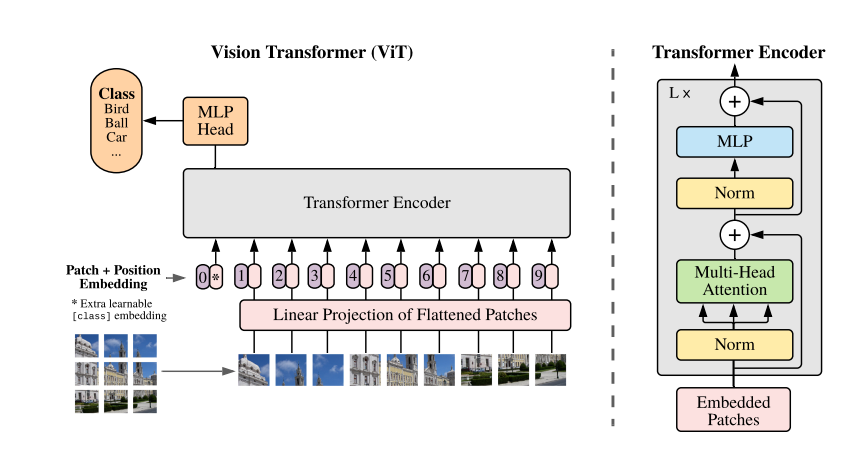
\includegraphics[width=\linewidth]{images/fig.png}
	\caption{
		Vision Transformer model overview.}
	\vspace{-2mm}
\end{figure}

\section{Introduction}
Transformer\cite{attentionneed} architecture is the model of choice in natural language processing. In computer vision, however, Convolutional Neural Network is dominant. Due to the success of Transformer, there is some works try to replace some convolutional layers to self-attention.

On the other hand, Vision Transformer\cite{transformerimage} apply standard Transformer directly to images, without any Convolutional layers. This model achieves excellent results in transfer learning based on pretraining with a large dataset(e.g. ImageNet-21k).

In this report, We summarize Vision Transformer paper\cite{transformerimage} focused on its architecture.

\section{Multihead self-attention}
self-attention generate Key, Value, Query vector from input vector. the size of matrix $U$ is $(D\times 3D_k)$ when an input sequence is $(N\times D)$
$$
[\textbf{q},\textbf{k},\textbf{v}] = \textbf{z}\textbf{U}_{qkv}
$$

The attention weights is similarity between query and key.
$$
A = \texttt{softmax}(\textbf{qk}^T/\sqrt{D_h})
$$
Output vector is product of attention weights and value.
$$
SA(\textbf{z}) = A\textbf{v}
$$

Multihead self-attention(MSA) is running $k$ self-attention operations, combining them, and apply linear projection.

$$
MSA(\textbf{z}) = [SA_1(z);SA(z);\cdots;SA_k(z)]\textbf{U}_{msa}
$$

\section{Vision Transformer}
model architecture is shown in Figure \ref{fig:modelarch}. The image was reshaped from $(H\times W \times C)$ into $(N\times (P^2 \cdot C))$, where H, W, and C is height, width, and channel of the image, $(P\times P)$ is resolution of patch, and N is the number of patches. A flattened patch passes through a D-dimensional vector to become a patch embedding vectors.

Position embeddings are added to the patch embedding. They use standard learnable 1D vector for position embeddings.

Additionally, There are extra learnable class embedding similar to BERT's class token.

The Transformer encoder consists of multiheaded self-attention(MSA) and MLP blocks. Layernorm(LN) is applied before every block.
$$
\textbf{z}_0 =[\textbf{x}_{class};\textbf{x}_p^1E;\textbf{x}_p^2E;\cdots \textbf{x}_p^NE;] + E_{pos} 
$$
$$
\textbf{z}'_l = MSA(LN(\textbf{z}_{l-1})) + z_{l-1} 
$$
$$
\textbf{z}_l = MLP(LN(\textbf{z}_{l-1})) + z_{l} 
$$
$$
y=LN(\textbf{z}_L^0)
$$

Transformer has much lass inductive bias than CNNs. only MLP layers are local and translationally equivariant.

They pretrain Vision Transformer using large datasets, and fine tune to smaller tasks. this network can handle arbitrary sequence length. however, when fine-tuning with higher resolution image than pre-training, position embeddings may no longer meaningful. They perform interpolation to the position embedding.

The details of the model variants are shown in Table \ref{tab:modelvariants}. For instance, ViT-L/16 means the large variant with $16\times16$ patch size. Large and Huge model pretrained with large dataset(JFT, Imagenet 21k) achieve better performance in popular image classification benchmarks(e.g. ImageNet, CIFAR-100, VTAB) while took less compute to pre-train than state-of-the art.



\subsection{Pre-training data requirements}
Transformer\cite{attentionneed} is modest when pretrained with smaller dataset due to have fewer inductive biases than CNN. however, ViT performs better when pretrained with large dataset such as JFM-300M than ResNet. Additionally, ViT uses approximately $2-4\times$ less compute to attain the same performance.

\section{Conclusion}
ViT is direct application of Transformer architectures to image classification. This model achieve better performance when pretrained with large dataset than CNN model or Big Transfer\cite{bit}, Additionally, this model is cheaper to pre-train.

\begin{table}[]
\centering
\begin{tabular}{llllll}
\hline
Model     & Layers & Hidden D & MLP size & Heads & Params \\ \hline
ViT-Base  & 12     & 768      & 3072     & 12    & 86M    \\
ViT-Large & 24     & 1024     & 4096     & 16    & 307M   \\
ViT-Huge  & 32     & 1280     & 5120     & 16    & 632M   \\ \hline
\end{tabular}
\caption{Details of Vision Transformer model variants.}
\label{tab:modelvariants}
\end{table}

\newpage
\bibliography{egbib}

\end{document}
